\documentclass[a4paper]{article}
\usepackage{graphicx}
\usepackage{siunitx}
\usepackage{csvsimple}
\usepackage{multirow}
\usepackage{booktabs}
\usepackage{amsmath,amsfonts,mathtools}
\usepackage[margin=3cm]{geometry}
\usepackage{footmisc}

    \begin{document}
        \section{Implementation of Flip-Flop D and SR Latch with discrete logic gates}
        Using the schematic on Figure \ref{fig:Schem} the logic gates were implemented on a PCB.
        
        \begin{figure}[h!]
            \begin{center}
                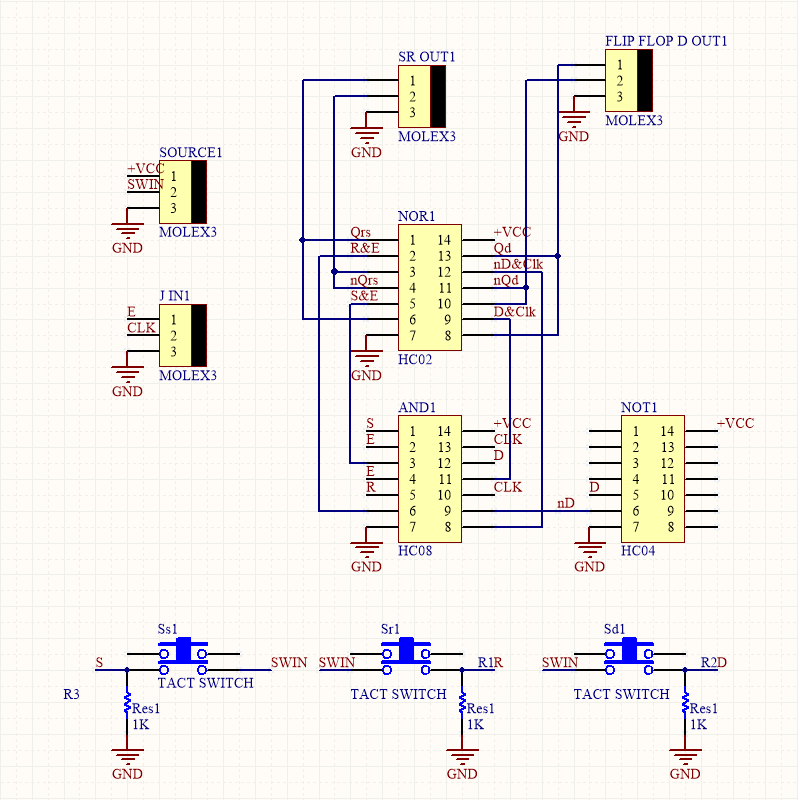
\includegraphics[width=\linewidth]{e6Schem.png}
                \caption{Schematic of the  SR Latch (on the left) and Flip-Flop D (on the right)}
            \end{center}
            \label{fig:Schem}
        \end{figure}

        The resulting circuits were tested and compared to their resulting counterparts as shown in
        Table \ref{tab:e6t1} and Table \ref{tab:e6t2}.

        \begin{table}[ht]
            \begin{center}
                \begin{tabular}{|l|l|r|r|r|r|r|r|c|}
    \toprule
    Symbol  &Parameter  &\multicolumn{3}{|c|}{74HC74}&\multicolumn{3}{|c|}{Experimental}&Unit\\
            &           &   MIN&NOM&MAX&MIN&NOM&MAX&\\
    \midrule
    $V_{CC}$&Supply Voltage&2&5&6&1.5&5&  &V\\
    $V_{IH}$&High-level input voltage&3.15&$-$&$-$&2.64&$-$&$-$&V\\
    $V_{IL}$&Low-level input voltage&$-$&$-$&1.35&$-$&$-$&2.57&V\\
    $V_{I}$ &Input voltage&0&$-$&$V_{CC}$&0&$-$&$V_{CC}$&V\\
    $V_{O}$ &Output voltage&0&$-$&$V_{CC}$&-0.2&$-$&$V_{CC}$&V\\
    $\Delta t / \Delta v$&  Input rise and fall time&$-$&$-$&0.5&$-$&$-$&16.05&$\mu$s\\
    \bottomrule
\end{tabular}
\caption{Operating Conditions comparison}
                \label{tab:e6t1}
            \end{center}
        \end{table}
        \begin{table}[ht]
            \begin{center}
                \begin{tabular}{|l|l|r|r|r|r|r|r|c|}
    \toprule
    Symbol  &Parameter  &\multicolumn{3}{|c|}{74HC74}&\multicolumn{3}{|c|}{Experimental}&Unit\\
            &           &   MIN&TYP&MAX&MIN&TYP&MAX&\\
    \midrule
    $V_{OH}$&High-level output voltage&3.84&4.3&$-$&  &  &$-$&V\\
    $V_{OL}$&Low-level output voltage &$-$&0.17&0.4&$-$&  &  &V\\
    \bottomrule
\end{tabular}
\caption{Electrical Characteristics comparison at $V_{CC}$=4.5V}
                \label{tab:e6t2}
            \end{center}
        \end{table}
    \end{document}